\documentclass[]{article}
\usepackage{graphicx}
\usepackage{enumitem}


\title{Architecture Report}
\author{KTH Group 2} % Please don't add names!

\begin{document}

\maketitle

\section*{Architecture of the Application}
	\begin{figure}[h]
	\centering
	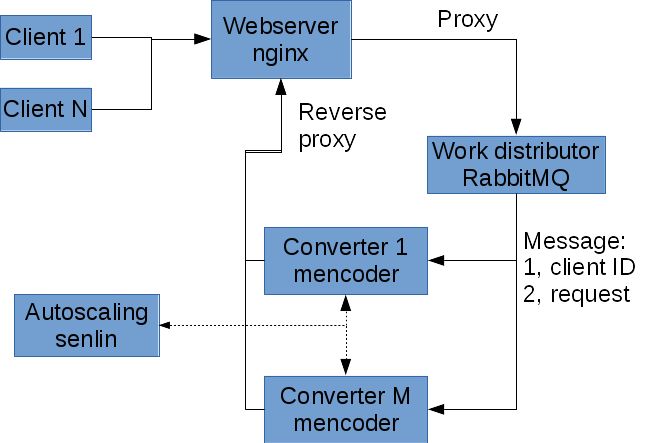
\includegraphics[width=\linewidth]{arch_diagram}
	\caption{}
	\label{fig:arch_diagram}
	\end{figure}

	\begin{itemize}
	\item No files are stored in the service.
	\item The requests are relayed from the webserver to the work distributor, a distributed message queue.
	\item A job consists of three parts:
	\begin{enumerate}
	\item Send the video from the client to the worker, through proxy server.
	\item The worker process the video.
	\item The worker sends back the converted video to the client, through proxy server
	\end{enumerate}
	\item The senlin module scales the number of running VMs, based on predefined policies.
	\end{itemize}

\section*{Component Overview}
	\begin{figure}[h]
	\centering
	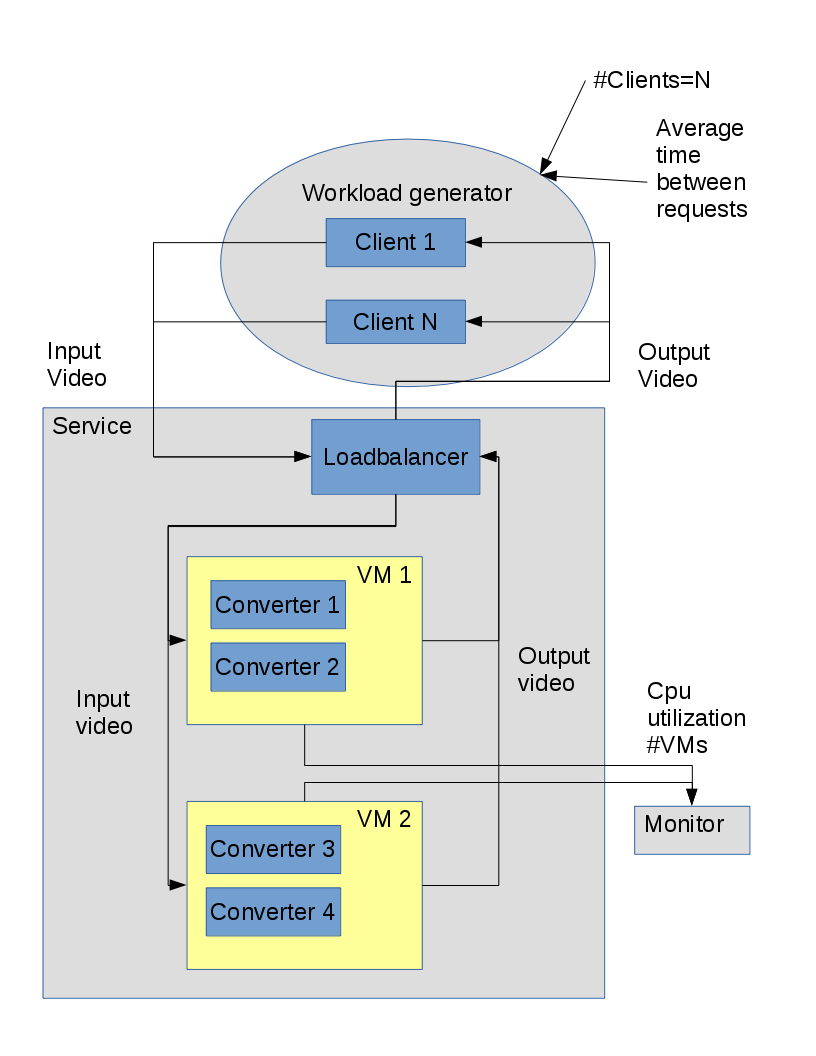
\includegraphics[width=\linewidth]{system_diagram}
	\caption{}
	\label{fig:system_diagram}
	\end{figure}
\section*{Exposed Interfaces}
	\begin{figure}[h]
	\centering
	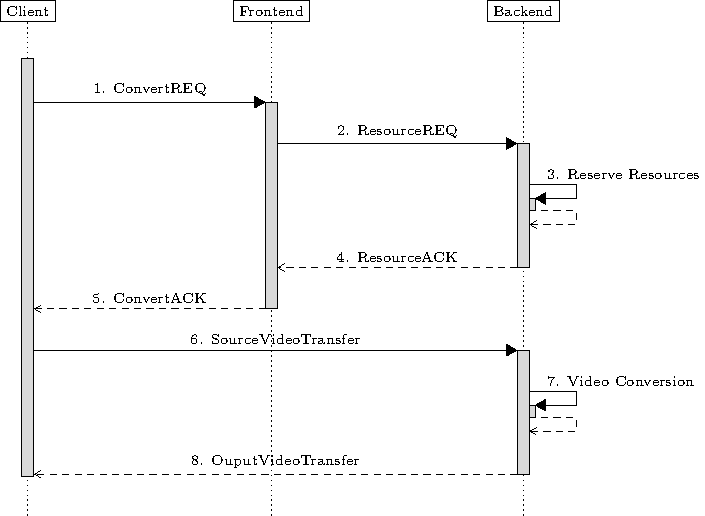
\includegraphics[width=\linewidth]{sequence_diagram}
	\caption{}
	\label{fig:sequence_diagram}
	\end{figure}
	
	Figure~\ref{fig:sequence_diagram} shows the sequence diagram, which consists of the following messages:
	\begin{enumerate}
		\item The client requests a video conversion from the frontend.
		\item The frontend requests the necesary resources from the backend.
		\item The backend reserves the necessary resources. 
		\item The backend acknowledges by providing a resource block.
		\item The frontend acknowledges that the video can be converted.
		\item The client can start transferring the source video.
		\item The backend converts the video to the desired format.
		\item The resulting video file is transfered back to the client. 
	\end{enumerate}
	
\section*{Technology Stack}
\section*{Scalability and Robustness}


\end{document}
